\documentclass[./main.tex]{subfiles}

\begin{document}

\begin{figure}[H]
\centering
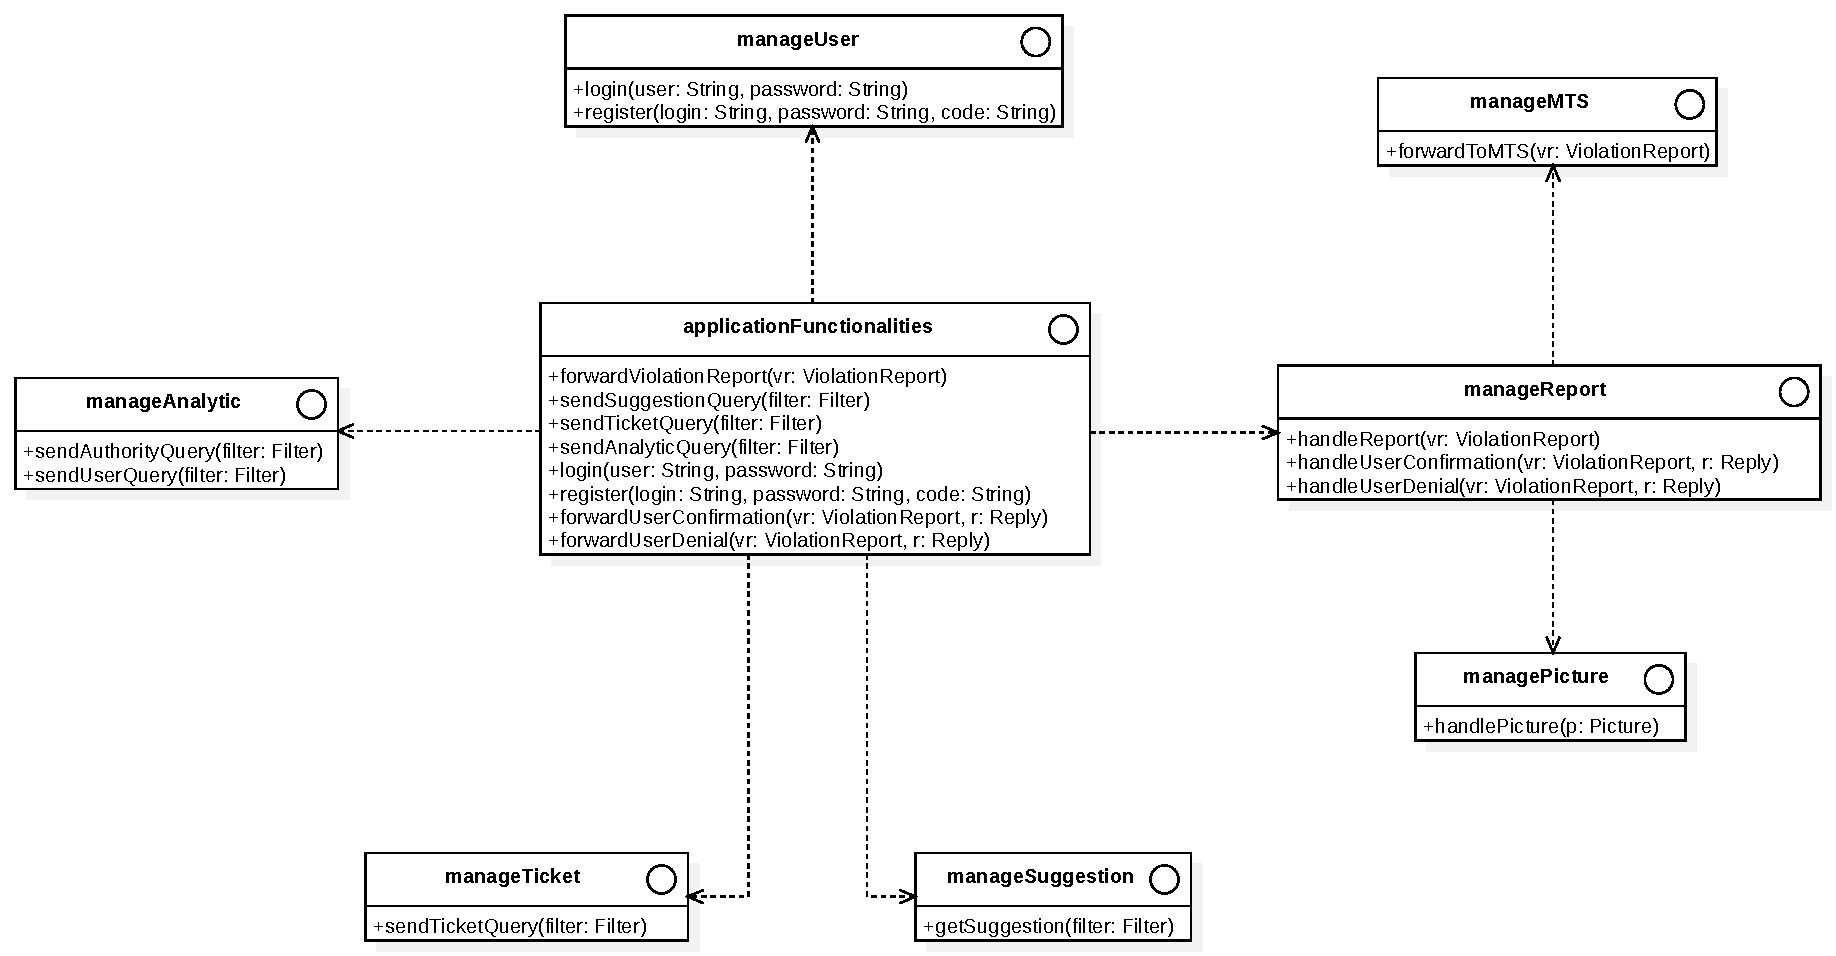
\includegraphics[width=\textwidth]{resources/interfaces_diagram}
\caption{Component interfaces}
\label{fig:interfaces}
\end{figure}

In the component interfaces diagram, the main interfaces described in the component diagram are better described. Not all the interfaces have been presented, because they are related to external services.\\\\
\textbf{applicationFunctionalities} interface is the main one, as it allows the communication between the users and all the services, exposing its methods to all of the main sub-components of ApplicationServer.
 
\begin{itemize}
\item
	\textbf{forwardViolationReport} is part of the subsystem which deals with reporting the violations. The argument of the method is a ViolationReport, consisting in an object which contains all the information related to the violation.
	
\item
	\textbf{sendSuggestionQuery}, \textbf{sendTicketQuery} and \textbf{sendAnalyticQuery} are different methods interacting with different services, but they all have in common the Filter parameter. Nevertheless, this is not to mean that all the filters are the same, indeed they depend on the type of user and service that is requested. They are expressed in the same formulation for compactness and to show their similarities. Take as an example sendAnalyticQuery: this method can be called by both common users and authorities to get data about the violations which, however, can get data in different levels of refinement and detail. The query filters' domain of the common user will be a subset of the one of the authority, but few differences apply to what the two types of users can do.
	
\item
	\textbf{login} and \textbf{register} accept as input the user name and password. Moreover, register can accept the code string, which identifies the user as authority or municipality user.
	
\end{itemize}

Most of the other interfaces are self explanatory at this point, as their name well describes their functionality, their parameters are the same as those just discussed, and so they are not furthermore described. Conversely, it is worth to describe the  \textbf{managePicture} interface, as it introduces a not yet described type of data. Here the method \textbf{handlePicture} deals with Picture which, however, is not a new type of data, but an object contained in ViolationReport consisting in the picture of the violation.

\end{document}